% Content for the test report for LSP-00-10

\subsection{API Aspect tests}

This test case exercises the LSP via the API Aspect only.

It verifies the ability to perform a variety of basic table scan queries.

Data for the test are primarily taken from the Object-like AllWISE (coadded) Source Catalog,
and the ForcedSource-like Multi-Epoch Photometry table,
except as noted below.

\subsubsection{Step 2}

The tests were performed primarily from an Apple Macbook Air computer running OS X 10.11.6,
connected to the Internet wirelessly at IPAC and other locations.
Queries requiring larger downloads were performed on an Apple iMac computing running OS X 10.11.6,
connected to the IPAC wired institutional network.

The tests were performed using Jupyter 5.4.1 on Python 3.6.1, and the notebook was accessed using version 11.1 of the Safari browser.

\subsubsection{Step 3}

A connection was established to the PDAC network environment using the NCSA VPN at \texttt{vpn.ncsa.illinois.edu}.

The \verb|dbserv| version 0 pseudo-TAP service was accessed at:

\begin{center}
\texttt{http://lsst-qserv-dax01.ncsa.illinois.edu:5000/db/v0/tap/sync}
\end{center}

\subsubsection{Step 4 --- Tests in the Jupyter notebook}

\textbf{Very small queries}

A target object was chosen near ( ra=4, dec=0 ):
\verb|source_id| ``\verb|0045p000_ac51-034420|'', \verb|cntr| 45100001351034420, \verb|ra| 3.9967364, \verb|decl| 0.002037.

Since the \verb|cntr| attribute is not indexed, a search for a row matching this unique ID in the Object-like database,
or a search for rows matching this as the parent-object ID in the ForcedSource-like database,
will result in a table scan.
If combined with a spatial restriction, this table scan can be limited to a subset of the database shards maintained by Qserv.

Following the guidance in LDM-540,
although these queries scan up to the full number of rows in these two tables (758 million and 42 billion, respectively),
they return only a small amount of data in the end.

A series of increasing-diameter cone searches were done,
using the special Qserv spatial-restriction function \verb|qserv_areaspec_circle|,
to trace out the behavior of Qserv as the fraction of shards scanned increased.

The query texts were:
\texttt{SELECT cntr, ra, decl, w1mpro, w2mpro FROM wise\_00.allwise\_p3as\_psd WHERE qserv\_areaspec\_circle(3.9967364,0.002037,} $r$ \texttt{) AND cntr=45100001351034420} for the Object-like table, and
\texttt{SELECT cntr, cntr\_mf, ra, decl, mjd, w1mpro\_ep, w2mpro\_ep FROM wise\_00.allwise\_p3as\_mep WHERE qserv\_areaspec\_circle(3.9967364,0.002037,} $r$ \texttt{) AND cntr\_mf=45100001351034420} for the ForcedSource-like table,
where the radius $r$ is in degrees.

The queries were carried out for radii in powers of two from $1/1024$ through $64$, and for the half-sky radius $89.9$.
Finally, an all-sky version was carried out by omitting the \verb|qserv_areaspec_circle| function.

All the queries returned the same results: a single row in the case of the Object-like queries,
and 24 rows of forced photometry associated with that object for the ForcedSource-like queries.
Successfully completing the half-sky and all-sky ForcedSource queries via \verb|dbserv| required raising the \verb|webserv|
timeout from 30 minutes to two hours.

\begin{table}[h]
\centering
\begin{tabular}{r r r r}
Radius (deg.) & Sky Area (sq. deg.) & Object elapsed time (s) & ForcedSource elapsed time (s) \\ \hline
0.0010 & $3.00\times 10^{-6}$ & 0.54 & 0.83 \\
0.0020 & $1.20\times 10^{-5}$ & 0.22 & 0.33 \\
0.0039 & $4.79\times 10^{-5}$ & 0.22 & 0.35 \\
0.0078 & $1.92\times 10^{-4}$ & 0.22 & 0.37 \\
0.0156 & $7.67\times 10^{-4}$ & 0.21 & 0.40 \\
0.0313 & $3.07\times 10^{-3}$ & 0.22 & 0.41 \\
0.0625 & $1.23\times 10^{-2}$ & 0.21 & 1.03 \\
0.125 & $4.91\times 10^{-2}$ & 0.21 & 0.67 \\
0.25 & $1.96\times 10^{-1}$ & 0.22 & 0.46 \\
0.5 & $7.85\times 10^{-1}$ & 0.23 & 0.40 \\
1.0 & $3.14\times 10^{0}$ & 0.33 & 0.45 \\
2.0 & $1.26\times 10^{1}$ & 0.92 & 0.62 \\
4.0 & $5.02\times 10^{1}$ & 1.84 & 3.55 \\
8.0 & $2.01\times 10^{2}$ & 5.22 & 5.79 \\
16.0 & $7.99\times 10^{2}$ & 16.59 & 17.27 \\
32.0 & $3.13\times 10^{3}$ & 55.67 & 59.13 \\
64.0 & $1.16\times 10^{4}$ & 207.62 & 942.73 \\
89.9 & $2.06\times 10^{4}$ & 380.07 & 2365.89 \\
all-sky & $4.13\times 10^{4}$ & 929.33 & 4506.66
\end{tabular}
\caption{Table-scan results for small queries on Object- and ForcedSource-like tables}
\label{tab:lsp-00-10-simple-scan-timings}
\end{table}

\begin{figure}
  \centering
  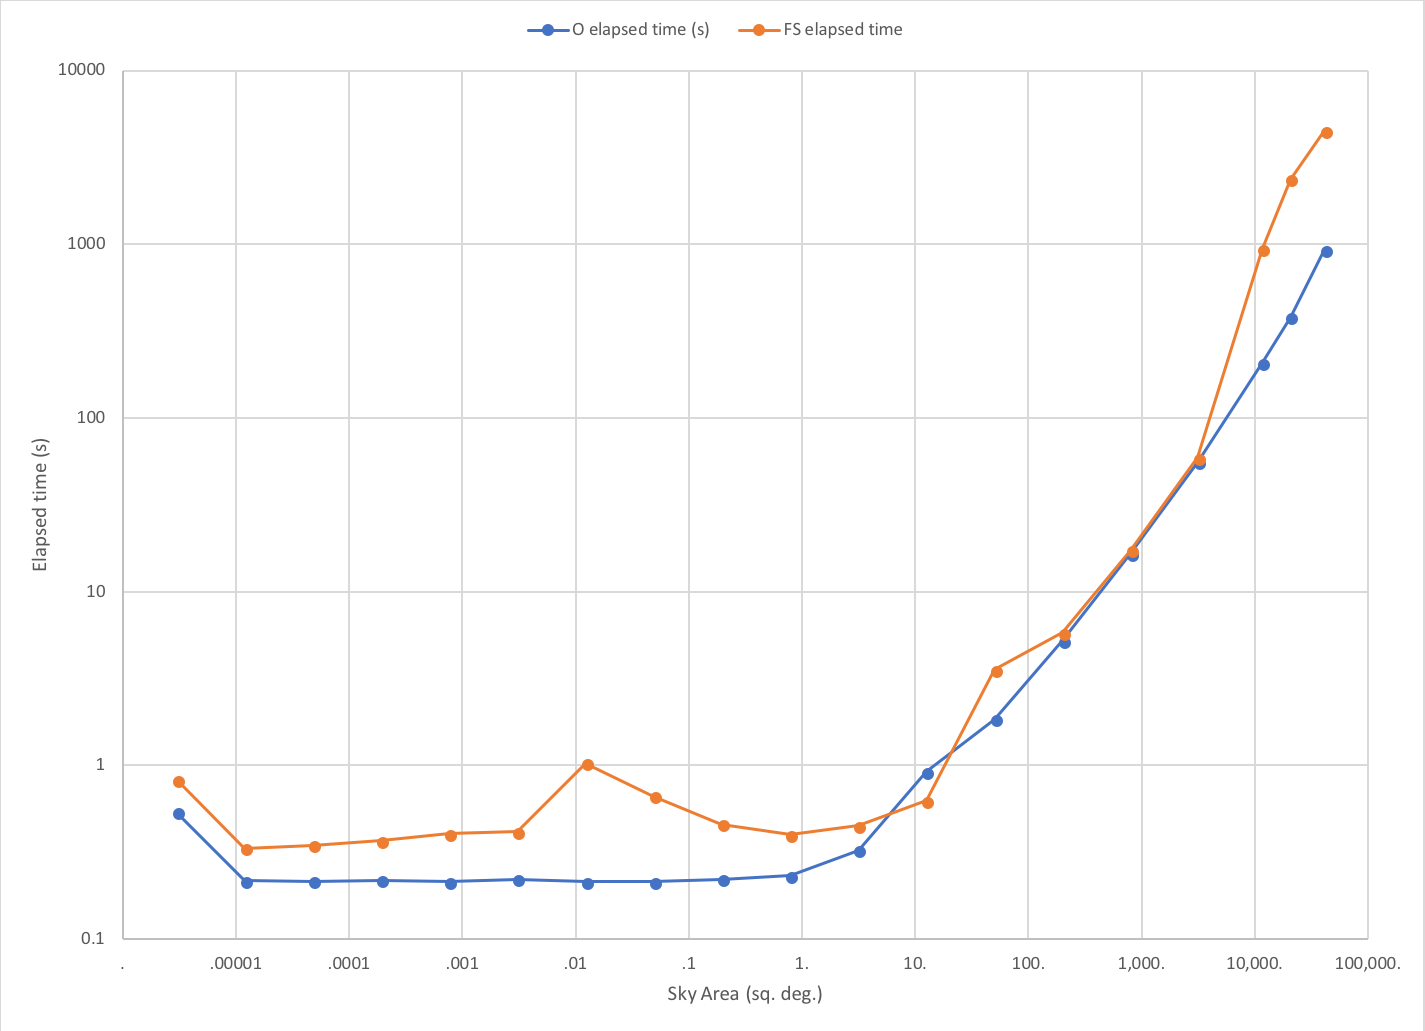
\includegraphics[width=4in]{lsp-00-10/SimpleScans.png}
  \caption{Query results for the Object-like AllWISE Source Catalog}
  \label{fig:lsp-00-10-simple-scan-plot}
\end{figure}

